% =========================================================================
% --- INICIO INPUT SEMANA 4 ---
% =========================================================================

\chapter{Semana 4: Levantamientos y Número de Rotación}

\section{Levantamientos de Aplicaciones en el Círculo}

\begin{definicion}[Levantamiento]
	Sea $f: S^1 \to S^1$ una aplicación continua. Una aplicación continua $F: \mathbb{R} \to \mathbb{R}$ se denomina un \textbf{levantamiento} de $f$ si el siguiente diagrama conmuta:
	$$ \pi \circ F = f \circ \pi $$
	donde $\pi: \mathbb{R} \to S^1$ es la proyección canónica $\pi(x) = e^{2\pi i x}$ (o en notación de cociente $\pi(x) = [x]$).
\end{definicion}

\begin{ejercicio}
	Sea $R_\theta: S^1 \to S^1$ la rotación, determinar todos sus levantamientos.
\end{ejercicio}
\begin{proof}[Solución]
	Sea $F: \mathbb{R} \to \mathbb{R}$ un levantamiento de $R_\theta$; i.e: $F \in C^0$ y $\pi \circ F = R_\theta \circ \pi \Rightarrow [F(x)] = R_\theta([x]) \Rightarrow [F(x)] = [x+\theta] \Rightarrow F(x) = x+\theta+k / k \in \mathbb{Z}$.
\end{proof}

\begin{proposicion}
	Sean $f: S^1 \to S^1 \in C^0$, $x_0 \in \mathbb{R} \land y_0 \in \pi^{-1}(f(\pi(x_0)))$. Entonces, existe una única aplicación continua $F: \mathbb{R} \to \mathbb{R}$ tal que: 
	i) $F(x_0) = y_0$, 
	ii) $\pi \circ F = f \circ \pi$ (P: Ejercicio).
\end{proposicion}
% \begin{proof}
	% 	Por la teoría clásica de espacios cubrientes (Topología Algebraica), dado que $\mathbb{R}$ es simplemente conexo (y por tanto su grupo fundamental es trivial) y $\pi: \mathbb{R} \to S^1$ es un recubrimiento, cualquier aplicación continua $f \circ \pi: \mathbb{R} \to S^1$ se puede levantar de forma única a una aplicación $\tilde{f}: \mathbb{R} \to \mathbb{R}$ una vez fijado el mapeo de un punto base $F(x_0) = y_0$, satisfaciendo $\pi \circ F = f \circ \pi$.
	% \end{proof}
\begin{proof}
	Por ahora, probaremos la unicidad: Sea $G: \mathbb{R} \to \mathbb{R}$ continua tal que también cumple las condiciones $\Rightarrow$ Sea $H: \mathbb{R} \to \mathbb{R} / H(x) = F(x) - G(x)$, continua $\Rightarrow H(\mathbb{R})$ es conexo. Y como $H(\mathbb{R}) \subseteq \mathbb{Z} \land H(x_0) = 0 \Rightarrow H(\mathbb{R}) = \{0\}$.
	Luego $F(x) = G(x) \Rightarrow F = G$.
	
	Ahora probaremos la existencia. Definimos: $F: \mathbb{R} \to \mathbb{R}, \quad x \mapsto F(x)$ 
	$$ F(x) = \begin{cases} 
		y & : \text{Si } \lfloor x_0 \rfloor \le x < \lfloor x_0 \rfloor + 1, \text{ donde } y \in \pi^{-1}(f(\pi(x))) \cap [y_0, y_0+1) \\ 
		y+k & : \text{Si } \lfloor x_0 \rfloor \le x^* < \lfloor x_0 \rfloor + 1, \text{ donde } x^* = x - k \, (k \in \mathbb{Z}) \land y = F(x^*) 
	\end{cases} $$
	
	\begin{figure}[htbp]
		\centering
		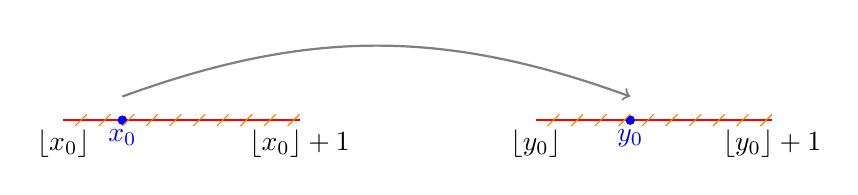
\begin{tikzpicture}[scale=1.5]
			\draw[thick, red] (0,0) -- (2,0);
			\draw[thick, red] (4,0) -- (6,0);
			
			\node[below] at (0,0) {$\lfloor x_0 \rfloor$};
			\node[below] at (2,0) {$\lfloor x_0 \rfloor + 1$};
			\node[below] at (4,0) {$\lfloor y_0 \rfloor$};
			\node[below] at (6,0) {$\lfloor y_0 \rfloor + 1$};
			
			\filldraw[blue] (0.5,0) circle (1pt) node[below] {$x_0$};
			\filldraw[blue] (4.8,0) circle (1pt) node[below] {$y_0$};
			
			\draw[->, thick, gray] (0.5, 0.2) to[bend left=20] (4.8, 0.2);
			
			% Rayado (Hatching)
			\foreach \x in {0.1, 0.3, ..., 1.9} {
				\draw[orange] (\x, -0.05) -- (\x+0.1, 0.05);
			}
			\foreach \x in {4.1, 4.3, ..., 5.9} {
				\draw[orange] (\x, -0.05) -- (\x+0.1, 0.05);
			}
		\end{tikzpicture}
	\end{figure}
	
	Es claro que $F(x_0) = y_0$ y que $\forall x \in \mathbb{R} \Rightarrow \exists k \in \mathbb{Z} / x^* = x - k \in [\lfloor x_0 \rfloor, \lfloor x_0 \rfloor + 1) \Rightarrow \pi \circ F(x) = \pi \circ F(x^*) = f \circ \pi(x^*) = f \circ \pi(x)$.
	Como $\pi$ es una aplicación continua y abta $\Rightarrow F \in C^0$.
\end{proof}

\begin{ejercicio}
	Sea $F: \mathbb{R} \to \mathbb{R}$ un levantamiento continuo de $f$. Mostrar que $F_k(x) = F(x) + k$ (con $k \in \mathbb{Z}$) es también un levantamiento de $f$.
\end{ejercicio}
\begin{proof}[Solución]
	Como $F \in C^0$, entonces $F_k(x) = F(x)+k \in C^0$. Además verificamos la conmutatividad:
	$$ (\pi \circ F_k)(x) = \pi(F(x)+k) = [F(x)+k] = [F(x)] = (\pi \circ F)(x) $$
	Dado que por hipótesis $\pi \circ F = f \circ \pi$, entonces $\pi \circ F_k = f \circ \pi$. Por ende, $F_k$ es un levantamiento de $f$.
\end{proof}

\begin{ejercicio}
	Sean $F, G$ levantamientos de $f$ y $g$ respectivamente. Mostrar que $F \circ G$ es un levantamiento de $f \circ g$.
\end{ejercicio}
\begin{proof}[Solución]
	Como $F, G \in C^0 \implies F \circ G \in C^0$. 
	Además evaluamos el diagrama conmutativo:
	$$ \pi \circ (F \circ G) = (\pi \circ F) \circ G = (f \circ \pi) \circ G = f \circ (\pi \circ G) = f \circ (g \circ \pi) = (f \circ g) \circ \pi $$
	Por lo tanto, la composición de los levantamientos levanta a la composición de las funciones.
\end{proof}

\begin{ejercicio}
	Si $f: S^1 \to S^1$ es un homeomorfismo y $F: \mathbb{R} \to \mathbb{R}$ un levantamiento de $f$. Mostrar que $F$ es un homeomorfismo.
\end{ejercicio}
\begin{proof}[Solución]
	\begin{itemize}
		\item \textbf{Inyectividad:} Sean $x, y \in \mathbb{R}$ tales que $F(x) = F(y)$. 
		Aplicando $\pi$: $\pi(F(x)) = \pi(F(y)) \implies f(\pi(x)) = f(\pi(y))$. Como $f$ es homeomorfismo (y por tanto inyectivo), $\pi(x) = \pi(y) \implies x - y = k \in \mathbb{Z}$.
		Pero al ser un levantamiento general de un homeomorfismo de $S^1$, se cumple que $F(x+k) = F(x) + \pm k$ (dependiendo si preserva o invierte orientación). Como $F(x) = F(y) \implies F(y+k) = F(y) \implies k = 0 \implies x = y$. Luego, $F$ es inyectivo.
		\item \textbf{Sobreyectividad:} Sea $y \in \mathbb{R}$. Por ser $f$ sobreyectiva, existe $[x] \in S^1$ tal que $f([x]) = [y]$.
		Entonces $\pi(F(x)) = \pi(y) \implies F(x) - y = k \in \mathbb{Z} \implies F(x) - k = y$.
		Utilizando la propiedad del levantamiento: $F(x-k) = F(x) - k$ (o similar si se invierte). Por lo tanto existe el elemento $x' = x-k \in \mathbb{R}$ tal que $F(x') = y$.
	\end{itemize}
	Como $F$ es biyectiva y continua (por definición de levantamiento), y su dominio $\mathbb{R}$ y codominio son el mismo espacio que cumple las condiciones topológicas estándar, su inversa también es continua. Así, $F$ es homeomorfismo.
\end{proof}

\begin{lema}
	Sea $f: S^1 \to S^1$ continua y $F: \mathbb{R} \to \mathbb{R}$ un levantamiento de $f$. Entonces existe un único entero $m \in \mathbb{Z}$ tal que:
	$$ F(x+1) = F(x) + m, \quad \forall x \in \mathbb{R} $$
	Además, si $F'$ es otro levantamiento de $f$, entonces se cumple la misma relación con el mismo $m$: $F'(x+1) = F'(x) + m$.
\end{lema}
\begin{proof}
	Observe que $\pi(F(x+1)) = f(\pi(x+1)) = f(\pi(x)) = \pi(F(x))$. 
	Por tanto, $F(x+1) - F(x) = k(x) \in \mathbb{Z}$.
	
	Definimos $h: \mathbb{R} \to \mathbb{Z}$ como $h(x) = F(x+1) - F(x)$. 
	Como $F$ es continua, $h$ es continua. Como $\mathbb{R}$ es conexo y la imagen de un conexo bajo una función continua es un conjunto conexo en el codominio, $h(\mathbb{R})$ debe ser un subespacio conexo de $\mathbb{Z}$. 
	Dado que el único subespacio conexo no vacío en $\mathbb{Z}$ es un punto (un conjunto unitario), la función $h(x)$ debe ser constante. Es decir, $h(\mathbb{R}) = \{m\}$ para algún $m \in \mathbb{Z}$.
	Por lo tanto, $F(x+1) - F(x) = m, \forall x \in \mathbb{R}$.
	
	Si $F'$ es otro levantamiento, entonces sabemos que $\pi(F'(x)) = \pi(F(x)) \implies F'(x) - F(x) = c \in \mathbb{Z}$. Como antes, por continuidad de $F$ y $F'$, esta diferencia $c$ debe ser una constante en todo $\mathbb{R}$.
	Evaluemos la relación para $F'$:
	$$ F'(x+1) - F'(x) = (F(x+1) + c) - (F(x) + c) = F(x+1) - F(x) = m $$
	Así, el entero $m$ depende únicamente de la función $f$ original.
\end{proof}

\begin{definicion}[Grado de una aplicación]
	Sean $f: S^1 \to S^1$ continua y $F: \mathbb{R} \to \mathbb{R}$ un levantamiento. El \textbf{grado} de $f$, denotado por $\text{deg}(f)$, se define como el único entero $m \in \mathbb{Z}$ del Lema anterior, de forma que:
	$$ F(x+1) = F(x) + m, \quad \forall x \in \mathbb{R} $$
	Anotamos $\text{deg}(f) = m$. La interpretación topológica de $\text{deg}(f)$ es la cantidad de "vueltas" netas que da la imagen de $f$ al recorrer el círculo una sola vez en el dominio.
\end{definicion}

\begin{ejemplo}
	Para $f([x]) = [2x]$, teníamos el levantamiento $F(x) = 2x$.
	$$ F(x+1) = 2(x+1) = 2x + 2 = F(x) + 2 $$
	Por lo tanto, $\text{deg}(f) = 2$.
\end{ejemplo}

\begin{observacion}
	Sabemos que si $f: S^1 \to S^1$ es un homeomorfismo, entonces su levantamiento $F: \mathbb{R} \to \mathbb{R}$ es un homeomorfismo de $\mathbb{R}$. 
	Como todo homeomorfismo en $\mathbb{R}$ debe ser estrictamente monótono (creciente o decreciente), $F$ es estrictamente monótono.
\end{observacion}

\begin{definicion}
	Sea $f: S^1 \to S^1$ un homeomorfismo. Decimos que $f$ \textbf{preserva orientación} si su levantamiento $F: \mathbb{R} \to \mathbb{R}$ es estrictamente creciente.
	Denotamos al conjunto de los homeomorfismos que preservan la orientación como $\text{Hom}_+(S^1)$.
\end{definicion}

\begin{proposicion}
	a) Si $f \in \text{Hom}_+(S^1) \Rightarrow \text{deg}(f) = 1$.
	
	Si $f \in \text{Hom}_-(S^1) \Rightarrow \text{deg}(f) = -1$.
\end{proposicion}
\begin{proof}
	Sea $F: \mathbb{R} \to \mathbb{R}$ un levantamiento de $f$. Como $f \in \text{Hom}_+(S^1)$, entonces $F$ es estrictamente creciente. Sea $m = \text{deg}(f)$. Tenemos: $F(x+1) = F(x) + m : \forall x \in \mathbb{R} \Rightarrow m > 0$. Como $m \in \mathbb{Z}$, supongamos que $m > 1$.
	
	Entonces, el diagrama conmuta: 
	
	\begin{figure}[htbp]
		\centering
		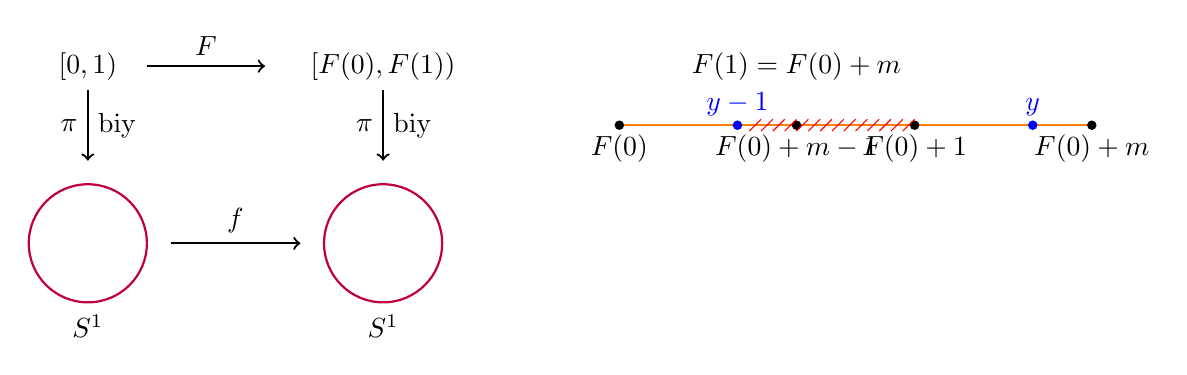
\begin{tikzpicture}[scale=1.5]
			% Diagrama de la izquierda
			\draw[thick, purple] (-1, -1.5) circle (0.5);
			\draw[thick, purple] (1.5, -1.5) circle (0.5);
			\draw[->, thick] (-0.3, -1.5) -- (0.8, -1.5) node[midway, above] {$f$};
			\draw[->, thick] (-1, -0.2) -- (-1, -0.8) node[midway, left] {$\pi$} node[midway, right] {biy};
			\draw[->, thick] (1.5, -0.2) -- (1.5, -0.8) node[midway, left] {$\pi$} node[midway, right] {biy};
			\node at (-1, 0) {$[0,1)$};
			\node at (1.5, 0) {$[F(0), F(1))$};
			\draw[->, thick] (-0.5, 0) -- (0.5, 0) node[midway, above] {$F$};
			\node at (-1, -2.2) {$S^1$};
			\node at (1.5, -2.2) {$S^1$};
			
			% Intervalo a la derecha
			\begin{scope}[shift={(3.5, -0.5)}]
				\draw[thick, orange] (0,0) -- (4,0);
				\node[below] at (0,0) {$F(0)$};
				\node[below] at (1.5,0) {$F(0)+m-1$};
				\node[below] at (2.5,0) {$F(0)+1$};
				\node[below] at (4,0) {$F(0)+m$};
				\node[above, blue] at (1, 0) {$y-1$};
				\node[above, blue] at (3.5, 0) {$y$};
				
				\filldraw[black] (0,0) circle (1pt);
				\filldraw[black] (1.5,0) circle (1pt);
				\filldraw[black] (2.5,0) circle (1pt);
				\filldraw[black] (4,0) circle (1pt);
				\filldraw[blue] (1,0) circle (1pt);
				\filldraw[blue] (3.5,0) circle (1pt);
				
				% Rayado
				\foreach \x in {1.1, 1.2, ..., 2.4} {
					\draw[red] (\x, -0.05) -- (\x+0.1, 0.05);
				}
			\end{scope}
			
			\node at (5, 0) {$F(1)=F(0)+m$};
		\end{tikzpicture}
	\end{figure}
	
	Luego, como: $\pi \circ F = f \circ \pi$.
	
	Entonces: como $y \neq y-1 \Rightarrow \exists x_1, x_2 \in [0,1)$ distintos / $F(x_1) = y, F(x_2) = y-1$.
	
	Luego: $\underbrace{\pi \circ F(x_1)}_{f \circ \pi(x_1)} = \pi(y-1) = \pi(y) = \underbrace{\pi \circ F(x_2)}_{f \circ \pi(x_2)}$.
	
	Luego, como $f$ es biy $\Rightarrow \pi(x_1) = \pi(x_2) \Rightarrow x_1 - x_2 \in \mathbb{Z} - \{0\} \quad (\rightarrow \leftarrow)$.
\end{proof}

\begin{ejercicio}
	Mostrar que $\text{deg}(f \circ g) = \text{deg}(f) \cdot \text{deg}(g)$ con $f, g \in \text{Hom}_+(S^1)$. ¿Es válido para $f, g$ continuas?
\end{ejercicio}
\begin{proof}[Solución]
	Como $f, g \in \text{Hom}_+(S^1)$, tienen grado 1. Sus levantamientos $F, G$ cumplen $F(x+1)=F(x)+1$ y $G(x+1)=G(x)+1$.
	Evaluando en la composición $F \circ G$ (la cual es un levantamiento de $f \circ g$):
	$$ (F \circ G)(x+1) = F(G(x+1)) = F(G(x)+1) = F(G(x)) + 1 = (F \circ G)(x) + 1 $$
	Por lo tanto $\text{deg}(f \circ g) = 1 = 1 \cdot 1 = \text{deg}(f) \cdot \text{deg}(g)$.
	
	Para $f,g$ funciones continuas generales con $\text{deg}(f)=m$ y $\text{deg}(g)=n$:
	$$ (F \circ G)(x+1) = F(G(x+1)) = F(G(x)+n) $$
	Utilizando la propiedad iterativamente: $F(y+n) = F(y) + n \cdot m$. 
	Entonces, $F(G(x)+n) = F(G(x)) + n \cdot m = (F \circ G)(x) + mn$.
	Así, la propiedad $\text{deg}(f \circ g) = \text{deg}(f) \cdot \text{deg}(g)$ es válida para todas las funciones continuas en $S^1$.
\end{proof}

\begin{proposicion}
	Sea $f: S^1 \to S^1 \in C^0 / \text{deg}(f) = m \neq 1$. Entonces $f$ posee un levantamiento $\tilde{F}: \mathbb{R} \to \mathbb{R}$ tal que $\tilde{F}(p) = p$, para algún $p \in [-1/2, 1/2]$.
\end{proposicion}
\begin{proof}
	Sea $F$ un levantamiento de $f$ consideremos $G: \mathbb{R} \to \mathbb{R}, x \mapsto G(x) = F(x) - x$.
	Tenemos: 
	$G(-1/2) = F(-1/2) + 1/2$
	$G(1/2) = F(1/2) - 1/2$
	También: $F(1/2) = F(-1/2+1) = F(-1/2)+m$
	$\Rightarrow F(1/2) - 1/2 = F(-1/2) - 1/2 + m = F(-1/2) + 1/2 - 1 + m$
	$\Rightarrow G(1/2) = G(-1/2) + m - 1$
	
	Supongamos: $m > 1$.
	
	\begin{figure}[htbp]
		\centering
		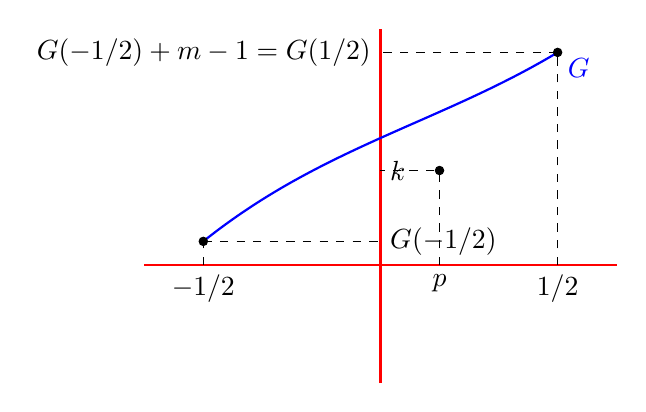
\begin{tikzpicture}[scale=1.5]
			\draw[thick, red] (-2,0) -- (2,0);
			\draw[thick, red] (0,-1) -- (0,2);
			
			\node[below] at (-1.5,0) {$-1/2$};
			\node[below] at (0.5,0) {$p$};
			\node[below] at (1.5,0) {$1/2$};
			
			\draw[blue, thick] (-1.5, 0.2) .. controls (-0.5, 1) and (0.5, 1.2) .. (1.5, 1.8) node[right, yshift=-0.2cm] {$G$};
			
			\draw[dashed, black] (-1.5, 0) -- (-1.5, 0.2);
			\draw[dashed, black] (1.5, 0) -- (1.5, 1.8);
			
			\draw[dashed, black] (-1.5, 0.2) -- (0, 0.2) node[right] {$G(-1/2)$};
			\draw[dashed, black] (0.5, 0) -- (0.5, 0.8) -- (0, 0.8) node[right] {$k$};
			\draw[dashed, black] (1.5, 1.8) -- (0, 1.8) node[left] {$G(-1/2)+m-1 = G(1/2)$};
			
			\filldraw[black] (0.5, 0.8) circle (1pt);
			\filldraw[black] (-1.5, 0.2) circle (1pt);
			\filldraw[black] (1.5, 1.8) circle (1pt);
		\end{tikzpicture}
	\end{figure}
	
	$\exists k \in \mathbb{Z} / k \in [G(-1/2), G(1/2)]$. Luego por el T.V.I.: $\exists p \in [-1/2, 1/2] / G(p) = k \Rightarrow F(p) - p = k$.
	
	Consideremos: $\tilde{F}: \mathbb{R} \to \mathbb{R}, x \mapsto \tilde{F}(x) = F(x) - k$.
	Luego $\tilde{F}$ es un levantamiento de $f \Rightarrow \tilde{F}(p) = F(p) - k = p \quad \blacksquare$
\end{proof}

\begin{ejercicio}
	Mostrar que: $R_\theta$ y $R_\alpha$ son topológicamente conjugados $\iff \alpha \pm \theta \in \mathbb{Z}$
\end{ejercicio}
\begin{proof}[Solución]
	$(\Rightarrow)$ Sea $h: S^1 \to S^1$ homeomorfismo / $h \circ R_\theta = R_\alpha \circ h$. Como $h \in \text{Hom}(S^1) \Rightarrow$ Sea $H: \mathbb{R} \to \mathbb{R}$ levantamiento de $h$, luego: $H(x+1) = H(x) + d \quad (d = \pm 1)$.
	
	Luego: Para $x \in \mathbb{R} \Rightarrow \pi \circ H(x+\theta) = [H(x+\theta)] = h([x+\theta]) = h \circ R_\theta([x]) = R_\alpha \circ h([x]) = R_\alpha([H(x)]) = [H(x)+\alpha] \Rightarrow H(x+\theta) = H(x) + \alpha + m / m \in \mathbb{Z}$.
	
	AFIR: $H(x+n\theta) = H(x) + n\alpha + nm$
	Hemos probado que para $n=1$ es válido.
	Por I.M: Sup: Es válido para "$n$":
	$$ H(x+(n+1)\theta) = H((x+n\theta)+\theta) =\newline H(x+n\theta) + \alpha + m = H(x) + n\alpha + nm + \alpha + m $$$$= H(x) + (n+1)\alpha + (n+1)m $$
	Luego, es válido $\forall n \in \mathbb{N}$.
	
	AFIR: $\exists M > 0 / \forall x \in \mathbb{R}: |H(x) - dx| \le M$.
	Sea $F: \mathbb{R} \to \mathbb{R} / F(x) = H(x) - dx$. Luego: $F(x+1) = H(x+1) - d(x+1) = H(x) + d - dx - d = H(x) - dx = F(x) \Rightarrow F(x+1) = F(x) : \forall x \in \mathbb{R}$.
	Y como es continua, y el intervalo $[0,1]$ es compacto $\Rightarrow F([0,1])$ es compacto. En particular acotado.
	
	Luego: Tomemos $x \in \mathbb{R} \Rightarrow |H(x+n\theta) - d(x+n\theta)| = |H(x) + n\alpha + nm - dx - dn\theta| \Rightarrow \left| \frac{H(x)-dx}{n} + m + \alpha - d\theta \right| \le \frac{M}{n}$, con $x$ fijo. Tomando límite $n \to \infty$: $m + \alpha - d\theta = 0 \Rightarrow \alpha - d\theta = -m \in \mathbb{Z}, d = \pm 1$.
	
	$(\Leftarrow)$ 
	$\cdot$ Si $\alpha + \theta = m \in \mathbb{Z}$. Sea $z \in S^1 / z = [x]$
	$\rightarrow$ Sea $h: S^1 \to S^1 / h(z) = -z \Rightarrow h \circ R_\theta(z) = h([x+\theta]) = [-x-\theta] = [-x+\alpha-m] = [-x+\alpha] = R_\alpha([-x]) = R_\alpha \circ h(z)$.
	
	$\cdot$ Si $\alpha - \theta = m \in \mathbb{Z}$. Sea $z \in S^1 / z = [x]$
	$\rightarrow$ Sea $h: S^1 \to S^1 / h(z) = z \Rightarrow h \circ R_\theta(z) = h([x+\theta]) = [x+\theta] = [x+\alpha-m] = [x+\alpha] = R_\alpha([x]) = R_\alpha \circ h(z)$.
\end{proof}


\section{Número de Rotación de Poincaré}

\begin{ejercicio}
	Si $f: S^1 \to S^1$ es un homeomorfismo que preserva orientación y $F: \mathbb{R} \to \mathbb{R}$ un levantamiento de $f$, entonces $\varphi: \mathbb{R} \to \mathbb{R}, x \mapsto \varphi(x) = F(x)-x$ es una aplicación periódica.
\end{ejercicio}
\begin{proof}[Solución]
	Sea $\varphi(x+1) = F(x+1) - (x+1) = F(x)+1 - (x+1) = F(x) - x = \varphi(x)$.
\end{proof}

\begin{ejercicio}
	Si $\text{deg}(f)=m$, entonces $\chi: \mathbb{R} \to \mathbb{R}, x \mapsto \chi(x) = F^m(x)-x$ es periódica, donde $F$ es un levantamiento de $f$.
\end{ejercicio}

\begin{ejercicio}
	Si $\text{deg}(f)=m$, entonces $F^k(x+1) = F^k(x) + m^k ; k \in \mathbb{Z}^+$. ¿ $F^k(x+p) = F^k(x) + p \cdot m^k$ ? ($p \in \mathbb{Z}^+$)
\end{ejercicio}
\begin{proof}[Solución (para ambos ejercicios anteriores)]
	Como $F(x+1) = F(x)+m$.
	Entonces: $F^2(x+1) = F(F(x+1)) = F(F(x)+m) = F(F(x)) + m \cdot m = F^2(x) + m^2$. De manera análoga: $F^k(x+1) = F^k(x) + m^k ; k \in \mathbb{Z}^+$.
	Luego: $F^k(x+2) = F^k(x+1+1) = F^k(x+1)+m^k = F^k(x)+m^k+m^k = F^k(x)+2m^k$. De manera análoga: $F^k(x+n) = F^k(x) + n \cdot m^k : \forall n \in \mathbb{Z}^+$.
	Luego: $\chi(x+1) = F^m(x+1) - (x+1) = F^m(x) + m^m - x - 1 = (F^m(x) - x) + (m^m - 1) = \chi(x) + m^m - 1$. Como $1 \neq 0 \Rightarrow m^m = 1 \Rightarrow m = 1$.
\end{proof}

\begin{proposicion}
	Sea $f: S^1 \to S^1$ un homeomorfismo que preserva orientación y $F: \mathbb{R} \to \mathbb{R}$ un levantamiento de $f$. Entonces, el límite $\lim_{n \to \infty} \frac{F^n(x)-x}{n}$ existe para todo $x \in \mathbb{R}$ y es independiente de $x$.
\end{proposicion}
\begin{proof}
	\textbf{P: Independencia:} Sean $x,y \in [0,1]$
	$$ \left| \frac{F^n(x)-x}{n} - \frac{F^n(y)-y}{n} \right| \le \frac{|F^n(x)-F^n(y)|}{n} + \frac{|x-y|}{n} \le \frac{1}{n} + \frac{|x-y|}{n} $$
	Luego, tomando $n \to +\infty \Rightarrow \lim_{n \to \infty} \frac{F^n(x)-x}{n} = \lim_{n \to \infty} \frac{F^n(y)-y}{n}$.
	
	\begin{figure}[htbp]
		\centering
		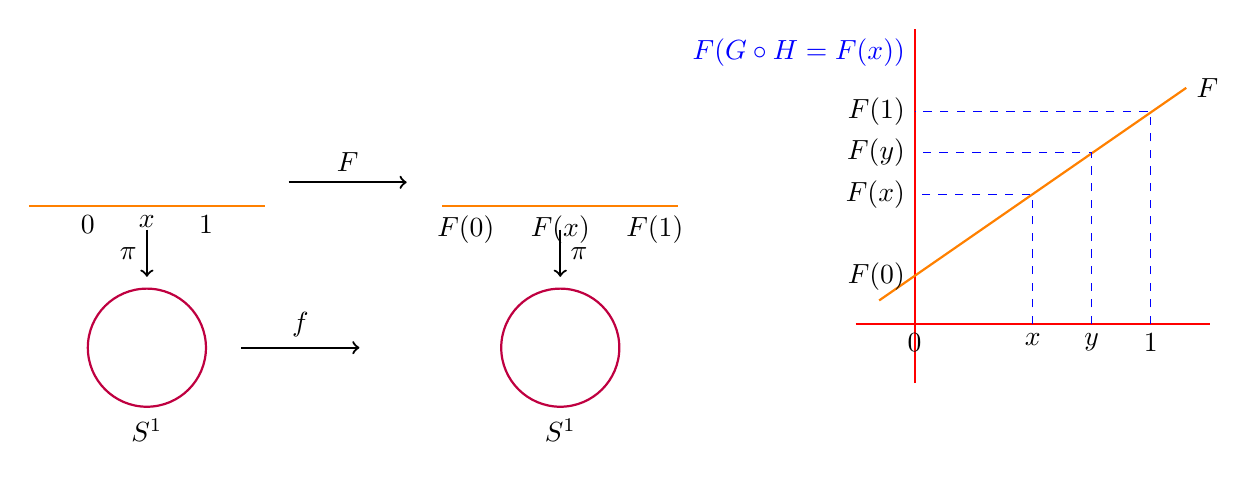
\begin{tikzpicture}[scale=1.5]
			% Lado Izquierdo
			\draw[thick, orange] (-1,0) -- (1,0);
			\node[below] at (-0.5,0) {$0$};
			\node[below] at (0,0) {$x$};
			\node[below] at (0.5,0) {$1$};
			\draw[->, thick] (0, -0.2) -- (0, -0.6) node[midway, left] {$\pi$};
			\draw[thick, purple] (0, -1.2) circle (0.5);
			\node at (0, -1.9) {$S^1$};
			
			\draw[->, thick] (1.2, 0.2) -- (2.2, 0.2) node[midway, above] {$F$};
			\draw[->, thick] (0.8, -1.2) -- (1.8, -1.2) node[midway, above] {$f$};
			
			% Lado Derecho
			\begin{scope}[shift={(2.5, 0)}]
				\draw[thick, orange] (0,0) -- (2,0);
				\node[below] at (0.2,0) {$F(0)$};
				\node[below] at (1,0) {$F(x)$};
				\node[below] at (1.8,0) {$F(1)$};
				
				\draw[->, thick] (1, -0.2) -- (1, -0.6) node[midway, right] {$\pi$};
				\draw[thick, purple] (1, -1.2) circle (0.5);
				\node at (1, -1.9) {$S^1$};
			\end{scope}
			
			% Gráfica
			\begin{scope}[shift={(6, -1)}]
				\draw[thick, red] (0, 0) -- (3, 0);
				\draw[thick, red] (0.5, -0.5) -- (0.5, 2.5);
				
				\node[below] at (0.5, 0) {$0$};
				\node[below] at (1.5, 0) {$x$};
				\node[below] at (2, 0) {$y$};
				\node[below] at (2.5, 0) {$1$};
				
				\draw[orange, thick] (0.2, 0.2) -- (2.8, 2) node[right, black] {$F$};
				
				\draw[dashed, blue] (1.5, 0) -- (1.5, 1.1) -- (0.5, 1.1) node[left, black] {$F(x)$};
				\draw[dashed, blue] (2, 0) -- (2, 1.45) -- (0.5, 1.45) node[left, black] {$F(y)$};
				\draw[dashed, blue] (0.5, 0.4) node[left, black] {$F(0)$} -- (0.5, 0.4);
				\draw[dashed, blue] (2.5, 0) -- (2.5, 1.8) -- (0.5, 1.8) node[left, black] {$F(1)$};
				
				\node[left, blue] at (0.5, 2.3) {$F(G \circ H = F(x))$};
			\end{scope}
		\end{tikzpicture}
	\end{figure}
	
	\textbf{Existencia: Ejercicio:} Sea $(a_n) \subseteq \mathbb{R}$ tal que: $a_{n+m} \le a_n + a_m + L \Rightarrow \{\frac{a_n}{n}\}_{n \in \mathbb{N}}$ es convergente, más aún $\lim_{n \to \infty} \frac{a_n}{n} = \inf \{ \frac{a_n}{n} : n \in \mathbb{N} \}$.
	
	Consideremos $a_n = F^n(x) - x ; x \in [0,1)$. AFIR: $a_{n+m} \le a_m + a_n + 1$. En efecto,
	$$ a_{m+n} = F^{m+n}(x) - x = F^m(F^n(x)) - x $$
	$$ = F^m(x+k) - (x+k) + (F^n(x) - x) + (F^m(F^n(x)) - F^m(x+k)) - (F^n(x) - x - k) $$
	Y como: $F^p(x+m) = F^p(x)+m \Rightarrow$
	$$ a_{m+n} = F^m(x) + k - (x+k) + F^n(x) - x + (F^m(F^n(x)) - F^m(x+k)) - (F^n(x) - (x+k)) $$
	$$ \le a_m + a_n + \overbrace{(F^m(F^n(x)) - F^m(x+k))}^{< 1} \Rightarrow a_{m+n} \le a_n + a_m + 1. $$
	Así, por el ejercicio: $\left\{ \frac{a_n}{n} \right\}_{n \in \mathbb{N}} = \left\{ \frac{F^n(x)-x}{n} \right\}_{n \in \mathbb{N}}$ es convergente.
\end{proof}

\begin{definicion}[Número de Rotación del Levantamiento]
	Sea $F: \mathbb{R} \to \mathbb{R}$ un levantamiento de $f \in \text{Hom}_+(S^1)$. Definimos el \textbf{número de traslación} del levantamiento $F$ como:
	$$ \rho(F) = \lim_{n \to \infty} \frac{F^n(x) - x}{n} $$
\end{definicion}

\begin{observacion}
	Si $F_1, F_2$ son dos levantamientos de la misma $f \in \text{Hom}_+(S^1)$, entonces difieren por un entero: $F_2(x) = F_1(x) + k$ para algún $k \in \mathbb{Z}$.
	Por inducción, $(F_2)^n(x) = (F_1)^n(x) + n k$.
	Evaluando el número de traslación:
	$$ \rho(F_2) = \lim_{n \to \infty} \frac{F_1^n(x) + nk - x}{n} = \lim_{n \to \infty} \left( \frac{F_1^n(x) - x}{n} + k \right) = \rho(F_1) + k $$
	Esto demuestra que el límite existe, pero su valor depende de la elección del levantamiento, difiriendo siempre por un número entero.
\end{observacion}

\begin{ejercicio}
	Mostrar que si $f \in \text{Hom}_+(S^1)$ y $F$ es un levantamiento de $f$, entonces $\rho(F^m) = m \rho(F)$ para todo $m \in \mathbb{Z}^+$.
\end{ejercicio}
\begin{proof}[Solución]
	Evaluemos por definición:
	$$ \rho(F^m) = \lim_{n \to \infty} \frac{(F^m)^n(x) - x}{n} = \lim_{n \to \infty} \frac{F^{mn}(x) - x}{n} $$
	Multiplicamos y dividimos por $m$:
	$$ \rho(F^m) = m \lim_{n \to \infty} \frac{F^{mn}(x) - x}{mn} $$
	Haciendo el cambio de variable $k = mn$, cuando $n \to \infty$, $k \to \infty$. Luego, el límite resultante es exactamente la definición de $\rho(F)$.
	$$ \rho(F^m) = m \lim_{k \to \infty} \frac{F^k(x) - x}{k} = m \rho(F) $$
\end{proof}

\begin{definicion}[Número de Rotación de Poincaré]
	Sea $f \in \text{Hom}_+(S^1)$. Definimos el \textbf{número de rotación} de $f$, denotado por $\rho(f)$, como la clase de equivalencia módulo 1 del número de traslación de cualquiera de sus levantamientos:
	$$ \rho(f) \equiv \rho(F) \pmod 1 $$
	Donde $\rho(f) \in [0, 1)$. Como demostramos que $\rho(F)$ solo difiere por enteros al cambiar de levantamiento, el valor fraccionario $\rho(f)$ está unívocamente determinado para $f$.
\end{definicion}

\begin{ejemplo}
	Consideremos $R_\theta: S^1 \to S^1$, $z \mapsto e^{2\pi i \theta}z$. 
	Un levantamiento de $R_\theta$ es $F(x) = x + \theta$.
	Calculamos sus iteraciones: $F^n(x) = x + n\theta$.
	Evaluamos el límite:
	$$ \rho(F) = \lim_{n \to \infty} \frac{x + n\theta - x}{n} = \lim_{n \to \infty} \frac{n\theta}{n} = \theta $$
	Por lo tanto, el número de rotación es $\rho(R_\theta) \equiv \theta \pmod 1$.
\end{ejemplo}

\begin{proposicion}
	Sean $f, g \in \text{Hom}_+(S^1)$ tal que $f$ y $g$ son conjugados topológicamente. Entonces, $\rho(f) = \rho(g)$.
\end{proposicion}
\begin{proof}
	Como $f$ y $g$ son top. conjugados, entonces $\exists h: S^1 \to S^1$ homeomorfismo tal que $h \circ f = g \circ h \Rightarrow h \circ f \circ h^{-1} = g$. Sean $F, G: \mathbb{R} \to \mathbb{R}$ y $H: \mathbb{R} \to \mathbb{R}$ levantamientos de $f, g$ y $h$ respectivamente.
	
	AFIR: $H \circ F \circ H^{-1}$ es un levantamiento de $g$. En efecto:
	$$ \pi \circ H \circ F \circ H^{-1} = h \circ \pi \circ F \circ H^{-1} = h \circ f \circ \pi \circ H^{-1} = h \circ f \circ h^{-1} \circ \pi = g \circ \pi $$
	
	Luego: $\rho(g) = \rho(H \circ F \circ H^{-1}) \pmod 1 = \lim_{n \to \infty} (H \circ F \circ H^{-1})^n(x) \pmod 1 = \lim_{n \to \infty} \frac{H \circ F^n \circ H^{-1}(x) - x}{n} \pmod 1$.\newline
	$= \lim_{n \to \infty} \left[ \frac{H(F^n(H^{-1}(x))) - F^n(H^{-1}(x))}{n} + \frac{F^n(H^{-1}(x)) - H^{-1}(x)}{n} + \frac{H^{-1}(x) - x}{n} \right] \pmod 1 \\= \rho(f) \Rightarrow \rho(g) = \rho(f)$
\end{proof}

\begin{ejercicio}
	Mostrar que un homeomorfismo $f \in \text{Hom}^+(S^1)$ tiene un punto fijo en $S^1 \iff \rho(f) \equiv 0 \pmod 1$.
\end{ejercicio}
\begin{proof}[Solución]
	$(\Rightarrow)$ Sea $[x] \in S^1$ un punto fijo de $f$. Entonces $f([x]) = [x]$. 
	Si $F$ es un levantamiento de $f$, evaluarlo en la coordenada $x$ da como resultado que la proyección no cambia: $\pi(F(x)) = \pi(x) \implies F(x) = x + m$ para algún entero $m \in \mathbb{Z}$.
	Analizando las iteraciones: $F^n(x) = x + nm$.
	Calculamos el número de traslación para ese $x$:
	$$ \rho(F) = \lim_{n \to \infty} \frac{F^n(x) - x}{n} = \lim_{n \to \infty} \frac{x + nm - x}{n} = m $$
	Como $\rho(F)$ es independiente del punto $x$, y $m \in \mathbb{Z}$, concluimos que $\rho(f) = m \pmod 1 \equiv 0 \pmod 1$.
	
	$(\Leftarrow)$ Sea $\rho(f) = 0 \pmod 1 \implies \rho(F) = m \in \mathbb{Z}$. Podemos elegir otro levantamiento $\tilde{F}(x) = F(x) - m$ tal que $\rho(\tilde{F}) = 0$.
	Por demostrar: existe $x \in \mathbb{R}$ tal que $\tilde{F}(x) = x$.
	Supongamos lo contrario. Como $\tilde{F}$ es continua, por el Teorema del Valor Intermedio, si no intersecta la identidad $y=x$, siempre estará por encima o siempre por debajo. Sin pérdida de generalidad, asumamos que $\tilde{F}(x) > x \implies \tilde{F}(x) - x > 0$.
	Como $[0,1]$ es un dominio compacto y $\tilde{F}(x)-x$ es estrictamente positiva y continua, alcanza un mínimo $\delta > 0$.
	Así, $\tilde{F}(x) \ge x + \delta$ para todo $x$. 
	Por inducción iterando la función estrictamente creciente: $\tilde{F}^n(x) \ge x + n\delta$.
	$$ \rho(\tilde{F}) = \lim_{n \to \infty} \frac{\tilde{F}^n(x) - x}{n} \ge \lim_{n \to \infty} \frac{n\delta}{n} = \delta > 0 $$
	Pero sabíamos que $\rho(\tilde{F}) = 0$, lo que genera una contradicción. Por lo tanto, debe existir un punto fijo $x$ para el levantamiento, el cual se proyecta en un punto fijo para $f$ en $S^1$.
\end{proof}

\begin{ejercicio}
	Si $f \in \text{Hom}^+(S^1)$, demostrar que $f$ posee un punto periódico de periodo $q \iff \rho(f) \equiv p/q \pmod 1$, con $(p,q)=1$.
\end{ejercicio}
\begin{proof}[Solución]
	Utilizaremos el resultado del ejercicio anterior.
	$f$ tiene un punto periódico de periodo $q \iff f^q$ tiene un punto fijo $\iff \rho(f^q) \equiv 0 \pmod 1$.
	Hemos demostrado que el número de traslación respeta la iteración: $\rho(F^q) = q \rho(F)$.
	Por lo tanto, la condición $\rho(f^q) \equiv 0 \pmod 1$ implica que el número de traslación original cumple: $q \rho(F) = p \in \mathbb{Z} \implies \rho(F) = p/q$.
	Así, $\rho(f) \equiv p/q \pmod 1$.
\end{proof}

\begin{ejercicio}
	Si $f, g \in \text{Hom}_+(S^1) / f \circ g = g \circ f$. Mostrar que $\rho(f \circ g) = \rho(f) + \rho(g) \pmod 1$.
\end{ejercicio}

\begin{ejercicio}
	Si $f \in \text{Hom}_+(S^1) / \rho(f) = p/q \quad (p,q \in \mathbb{Z}^+ \land (p,q)=1)$. Mostrar que todos los puntos periódicos de $f$ tienen periodo $q$.
\end{ejercicio}

\begin{ejercicio}
	Si $f \in \text{Hom}_+(S^1)$ tal que $\rho(f) \in \mathbb{Q} \pmod 1 \Rightarrow \Omega(f) = Per(f)$.
\end{ejercicio}

\begin{ejercicio}
	Si $f \in \text{Hom}_+(S^1) / \rho(f) \in \mathbb{Q} \pmod 1$ y $Per(f) = S^1$. Mostrar que $f$ es topológicamente conjugada a la rotación racional.
\end{ejercicio}

% =========================================================================
% --- FIN INPUT SEMANA 4 ---
% =========================================================================